\subsection{Third Research Question}
\label{sec:ResearchQuestion3}
The third research question of this project states:
\\
"How can the model be visualized to enforce explainability?"
\\\\
The proposed SCVM, modelling dynamic networks using Newtonian dynamics in Euclidean latent space, is specifically designed for enabling the creation of representations that can be visualized and are explainable.
The results presented in this section seek to evaluate to what extend this explainability is present, and what impact applying corrections and regularization has on the explainability of produced visualizations.


\subsubsection{Position and Drift Correction}
\label{sec:ResearchQuestion3:PositionCorrection}
The first investigation of explainability deals with the impact of implementing position and drift correction in the SCVM.
The SCVM without will fit its parameters in accordance to the intensities of interactions between nodes, meaning the model is \textit{only} concerned with the reciprocal distances between nodes at through time.
These distances are in themselves indifferent to where the center of the overall system is, and the drift of the entire system of nodes through latent space.
The animation in the link below shows the SCVM trained for 5000 epochs, fitted with 100 steps to the Resistance real dataset 1, see section \ref{sec:Data:RealData:RealDataset1}, without any correction at all.
\\
Notice that the bar on the bottom of the html page works as a slider, and dragging it will move the nodes according to time. 
Also, marking an area of the animation will fit the frame to that area, ie. zoom.
\begin{center}
\bluehref{https://tgml-bachelor-project.github.io/resistance-no-correction.html}{LINK: NO POSITION AND NO DRIFT CORRECTION}
\end{center}
\noindent
As can be seen, this animation shows a system of interacting nodes drifting in the latent space.
While the dynamic network of a game of Resistance is represented correctly in the animation, the fact that it is drifting in latent space makes understanding the dynamics of the system less straight forward.
In order to enforce explainability and make it easier to interpret the dynamics of the system, the starting positions are centered around origo, the coordinates (0,0), and drift is removed, as explained under section \ref{sec:Method:ProposedModel:PositionCorrection}.
Training the SCVM with position and drift correction yields the animation in the link below.
\begin{center}
\bluehref{https://tgml-bachelor-project.github.io/resistance-with-pos-drift-correction.html}{LINK: POSITION AND DRIFT CORRECTION}
\end{center}
\noindent
This corrected animation shows the exact same dynamics, but in a stable frame of the latent space, centered around origo, providing for a more interpretable animation.


\subsubsection{Rotation Correction}
\label{sec:ResearchQuestion3:RotationCorrection}
With the correction of positions and drift, the animations are more easily interpretable and serve a better foundation of being able to infer and explain what is going on in the given dynamic network.
As with positions and drift, the rotation of the given system does not impact the node pair distances, and can hence be neutralized as explained under section \ref{sec:Method:ProposedModel:RotationCorrection}.
An animation of the Resistance game, again trained for 5000 epochs, fitted with 100 steps, is shown in the link below:
\begin{center}
\bluehref{https://tgml-bachelor-project.github.io/resistance-with-pos-drift-rot-correction.html}{LINK: ROTATION CORRECTION}
\end{center}
\noindent
What this animation entails, while being distinct from but still similar to the one with position and drift correction applied, is a standardized system rotation in which the most movement happens along the x-axis, regardless of which dynamic network is modelled.

\subsubsection{Regularization}
\label{sec:ResearchQuestion3:Regularization}
In order to further enforce explainability with the visualizations of a given dynamic network, a regularization parameter is added as explained under section \ref{sec:Method:ProposedModel:Regularization}.
\\
The evaluation of the impact from applying various degrees of regularization is based on animations of the SCVM fitted to the Resistance game dataset as with the above results of corrections.
The animation shown in the link below is the SCVM trained for 5000 epochs, fitted to 100 steps, with correction of positions, drift, and rotation applied.
\begin{center}
\bluehref{https://tgml-bachelor-project.github.io/resistance-no-regu.html}{LINK: RESISTANCE GAME NO REGULARIZATION}
\end{center}
\\
The velocities in latent space for all nodes are free to change drastically between each step.
While the above animation visualizes how the 8 players and computer (P0) interact with each other over the duration of the game, their movements in latent space are to some extend changing drastically, seen by their shootings back and forth.
In order to limit this, with the goal of making inter-step changes less drastic, the model is regularized with values $\gamma = [10, 50, 200, 500]$:
\begin{align*}
    %&\bluehref{https://tgml-bachelor-project.github.io/resistance-regu5.html}{\text{LINK: RESISTANCE GAME WITH REGULARIZATION 5}} \\
    &\bluehref{https://tgml-bachelor-project.github.io/resistance-regu10.html}{\text{LINK: RESISTANCE GAME WITH REGULARIZATION 10}} \\
    &\bluehref{https://tgml-bachelor-project.github.io/resistance-regu50.html}{\text{LINK: RESISTANCE GAME WITH REGULARIZATION 50}} \\
    &\bluehref{https://tgml-bachelor-project.github.io/resistance-regu200.html}{\text{LINK: RESISTANCE GAME WITH REGULARIZATION 200}} \\
    &\bluehref{https://tgml-bachelor-project.github.io/resistance-regu500.html}{\text{LINK: RESISTANCE GAME WITH REGULARIZATION 500}}
\end{align*}
These animations show a reduction in the changes of velocity for each step. As such the regularization to some extend limits the drastic velocity changes of the nodes from one step to the next. 
\\
The impact that regularization is related much by the number of steps fitted by the SCVM to the data.
Below are animations for the Resistance game modelled with 1000 steps, with regularization $\gamma = 0$ and $\gamme = 250$.

\begin{align*}
    &\bluehref{https://tgml-bachelor-project.github.io/resistance-1000steps-no-regu.html}{\text{LINK: 1000 STEPS RESISTANCE GAME WITH REGULARIZATION 0}} \\
    &\bluehref{https://tgml-bachelor-project.github.io/resistance-1000steps-regu250.html}{\text{LINK: 1000 STEPS RESISTANCE GAME WITH REGULARIZATION 250}}
\end{align*}
Beyond the fact that the regularization has a more drastic impact on the animations of the 1000 steps fitted data, the higher number of steps also makes a big impact on how the nodes move in relation to each other.
An increased number of steps hence enhances the detail with which the dynamic network is represented.


\subsubsection{Animation Time-Resolution}
\label{sec:ResearchQuestion3:Lyon}
As a final evaluation of the explainability of the learned dynamics, the Lyon Primary School dataset, see real dataset 2 under section \ref{sec:Data:RealData:RealDataset3}, is modelled by the SCVM.
\\
This dataset has labels for all nodes, which tells an observer which school class each pupil belongs to, if not a teacher, and so can be interpreted with some added information. 
The links below show the same trained SCVM model dynamics for the Lyon dataset modelled, but with a different number of animation time points in the animation. 
Here, the impact of the number of animation time bins becomes clear as, while the animations are produced on the same learned model parameters, increasing the time-resolution directly yields a more detailed image of the dynamic network at any given point in time.  
\begin{align*}
    &\bluehref{https://tgml-bachelor-project.github.io/lyon-100.html}{\text{LINK: LYON PRIMARY SCHOOL 100 ANIMATION TIME POINTS}} \\
    &\bluehref{https://tgml-bachelor-project.github.io/lyon-2000.html}{\text{LINK: LYON PRIMARY SCHOOL 2000 ANIMATION TIME POINTS}} \\
    &\bluehref{https://tgml-bachelor-project.github.io/lyon-3000.html}{\text{LINK: LYON PRIMARY SCHOOL 3000 ANIMATION TIME POINTS}} \\
    &\bluehref{https://tgml-bachelor-project.github.io/lyon-5000.html}{\text{LINK: LYON PRIMARY SCHOOL 5000 ANIMATION TIME POINTS}}
\end{align*}
\noindent
This animation runs over a time span corresponding to 83 days. 
While presenting the dynamic network as one big cluster at some times, the animation clearly shows the groupings of some or more classes most of the time.
The teachers also seem to be interacting with one class each, for much of the animation, which inherently makes sense.

\begin{figure}[H]
    \centering
    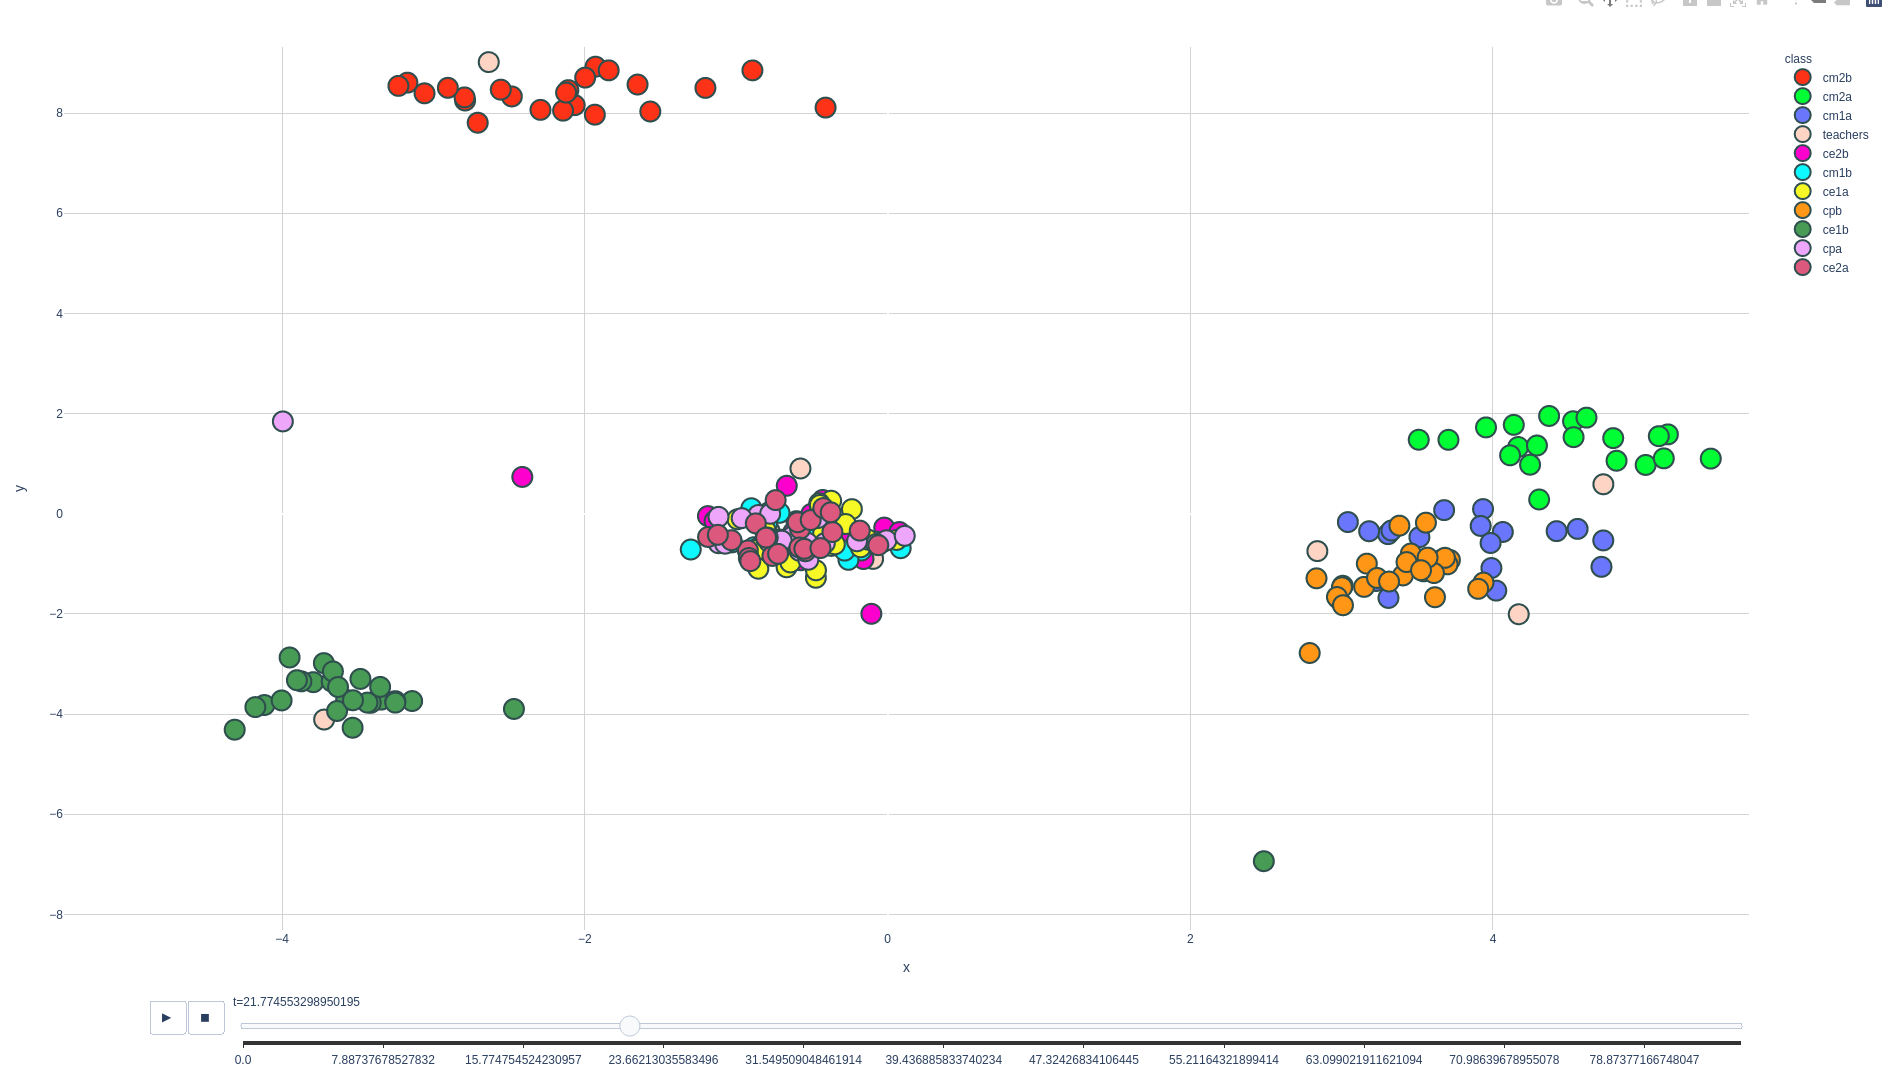
\includegraphics[width=\textwidth]{0_images/lyon_screenshot.png}
    \caption{Screenshot from the SCVM learned representation of the Lyon Primary School dynamic network data. Each color represents a different school class of pupils, while the teachers, colored sand, can be see near one class each in some cases.}
    \label{fig:LyonScreenshot}
\end{figure}